% Options for packages loaded elsewhere
\PassOptionsToPackage{unicode}{hyperref}
\PassOptionsToPackage{hyphens}{url}
\PassOptionsToPackage{dvipsnames,svgnames,x11names}{xcolor}
\documentclass[
  american,
  11pt,
  letterpaper,
]{article}
\usepackage{xcolor}
\usepackage[margin=1in]{geometry}
\usepackage{amsmath,amssymb}
\setcounter{secnumdepth}{-\maxdimen} % remove section numbering
\usepackage{iftex}
\ifPDFTeX
  \usepackage[T1]{fontenc}
  \usepackage[utf8]{inputenc}
  \usepackage{textcomp} % provide euro and other symbols
\else % if luatex or xetex
  \usepackage{unicode-math} % this also loads fontspec
  \defaultfontfeatures{Scale=MatchLowercase}
  \defaultfontfeatures[\rmfamily]{Ligatures=TeX,Scale=1}
\fi
\usepackage{lmodern}
\ifPDFTeX\else
  % xetex/luatex font selection
  \setmainfont[]{Latin Modern Roman}
  \setsansfont[]{Latin Modern Sans}
  \setmonofont[]{Latin Modern Mono}
\fi
% Use upquote if available, for straight quotes in verbatim environments
\IfFileExists{upquote.sty}{\usepackage{upquote}}{}
\IfFileExists{microtype.sty}{% use microtype if available
  \usepackage[]{microtype}
  \UseMicrotypeSet[protrusion]{basicmath} % disable protrusion for tt fonts
}{}
\makeatletter
\@ifundefined{KOMAClassName}{% if non-KOMA class
  \IfFileExists{parskip.sty}{%
    \usepackage{parskip}
  }{% else
    \setlength{\parindent}{0pt}
    \setlength{\parskip}{6pt plus 2pt minus 1pt}}
}{% if KOMA class
  \KOMAoptions{parskip=half}}
\makeatother
\usepackage{longtable,booktabs,array}
\newcounter{none} % for unnumbered tables
\usepackage{calc} % for calculating minipage widths
% Correct order of tables after \paragraph or \subparagraph
\usepackage{etoolbox}
\makeatletter
\patchcmd\longtable{\par}{\if@noskipsec\mbox{}\fi\par}{}{}
\makeatother
% Allow footnotes in longtable head/foot
\IfFileExists{footnotehyper.sty}{\usepackage{footnotehyper}}{\usepackage{footnote}}
\makesavenoteenv{longtable}
\usepackage{graphicx}
\makeatletter
\newsavebox\pandoc@box
\newcommand*\pandocbounded[1]{% scales image to fit in text height/width
  \sbox\pandoc@box{#1}%
  \Gscale@div\@tempa{\textheight}{\dimexpr\ht\pandoc@box+\dp\pandoc@box\relax}%
  \Gscale@div\@tempb{\linewidth}{\wd\pandoc@box}%
  \ifdim\@tempb\p@<\@tempa\p@\let\@tempa\@tempb\fi% select the smaller of both
  \ifdim\@tempa\p@<\p@\scalebox{\@tempa}{\usebox\pandoc@box}%
  \else\usebox{\pandoc@box}%
  \fi%
}
% Set default figure placement to htbp
\def\fps@figure{htbp}
\makeatother
\ifLuaTeX
\usepackage[bidi=basic,shorthands=off]{babel}
\else
\usepackage[bidi=default,shorthands=off]{babel}
\fi
\ifPDFTeX
\else
\babelfont{rm}[]{Latin Modern Roman}
\fi
\ifLuaTeX
  \usepackage{selnolig} % disable illegal ligatures
\fi
\setlength{\emergencystretch}{3em} % prevent overfull lines
\providecommand{\tightlist}{%
  \setlength{\itemsep}{0pt}\setlength{\parskip}{0pt}}
\usepackage{titlesec}
\usepackage{fancyhdr}
\usepackage{caption}
\usepackage{needspace}
\usepackage{fvextra}
\usepackage{float}
\AtBeginDocument{\hypersetup{allcolors=black}\floatplacement{figure}{H}}
\setmonofont[BoldFont={Latin Modern Mono}]{Latin Modern Mono}
\renewcommand{\texttt}[1]{{\ttfamily\fontsize{9.5}{11}\selectfont\hyphenchar\font=-1 #1}}
\titleformat{\section}{\large\bfseries}{\thesection}{0.5em}{}
\titleformat{\subsection}{\normalsize\bfseries}{\thesubsection}{0.5em}{}
\titlespacing*{\section}{0pt}{16pt}{7pt}
\titlespacing*{\subsection}{0pt}{11pt}{5pt}
\captionsetup{font=small,labelfont=bf,justification=raggedright,singlelinecheck=false}
\pagestyle{fancy}
\fancyhf{}
\fancyhead[L]{\small Open3DCP | Manuscript v1.2 preprint}
\fancyhead[R]{\small Schema v1.8 draft}
\fancyfoot[C]{\small\thepage}
\renewcommand{\headrulewidth}{0pt}
\setlength{\headheight}{15pt}
\setlength{\emergencystretch}{3em}
\widowpenalty=10000
\clubpenalty=10000
\brokenpenalty=10000
\renewcommand{\arraystretch}{1.12}
\raggedbottom
\makeatletter
\renewcommand{\maketitle}{\begingroup\parindent0pt
{\sffamily\bfseries\fontsize{21}{25}\selectfont\@title\par}
\vspace{9pt}{\large\@author\par}\vspace{4pt}
\endgroup}
\makeatother
\usepackage{bookmark}
\IfFileExists{xurl.sty}{\usepackage{xurl}}{} % add URL line breaks if available
\urlstyle{same}
\hypersetup{
  pdftitle={Open3DCP: A Public Data Schema for 3D Concrete Printing},
  pdfauthor={Nicholas Sonnentag},
  pdflang={en-US},
  colorlinks=true,
  linkcolor={black},
  filecolor={Maroon},
  citecolor={black},
  urlcolor={black},
  pdfcreator={LaTeX via pandoc}}

\title{Open3DCP: A Public Data Schema for 3D Concrete Printing}
\usepackage{etoolbox}
\makeatletter
\providecommand{\subtitle}[1]{% add subtitle to \maketitle
  \apptocmd{\@title}{\par {\large #1 \par}}{}{}
}
\makeatother
\subtitle{Recording composition, process, test context and provenance}
\author{Nicholas Sonnentag}
\date{15 September 2026}

\begin{document}
\maketitle

\textbf{Sunnyday Technologies, Wisconsin, USA}\\
ORCID: \href{https://orcid.org/0009-0002-1897-384X}{0009-0002-1897-384X}

\textbf{Manuscript v1.2: preprint. Not peer reviewed.}\\
Technical target: Open3DCP schema \textbf{v1.8 draft}, commit
\texttt{fa5fdd5} (15 September 2026 snapshot).\\
Original publication: 14 May 2026. Retained v1.0: 10 June 2026; v1.1: 30
July 2026. Revision: 15 September 2026.

\section{Abstract}\label{abstract}

Concrete test data need more than a strength value and a mix name. A
useful record also identifies the material, reporting basis, production
conditions, specimen and test. Open3DCP provides a public, flat column
vocabulary with companion tables for extrusion-based 3D concrete
printing. The v1.8 draft contains 279 data columns in its main table,
excluding the primary key. This revision explains the additions for
commercial premix identity, EN cement designations and aggregate size
fractions. It shows how to retain source quantities in kg/m³ while
deriving mass-percent values under stated accounting conditions. A
read-only audit examines 71 retained example rows from five
heterogeneous sources. These are conversion examples and aggregates, not
71 independent experiments or a validated training corpus. The audit
reproduces a mass-basis round trip and identifies incompatible grouping
in the earlier RILEM extraction; the previous quantitative anisotropy
conclusion is withdrawn. Common fields can make reporting and checking
easier, but do not establish experimental comparability, physical
performance or code compliance. The contribution is a documented
reporting method and an inspectable account of what conversion
preserves, changes and leaves unresolved.

\begin{figure}
\centering
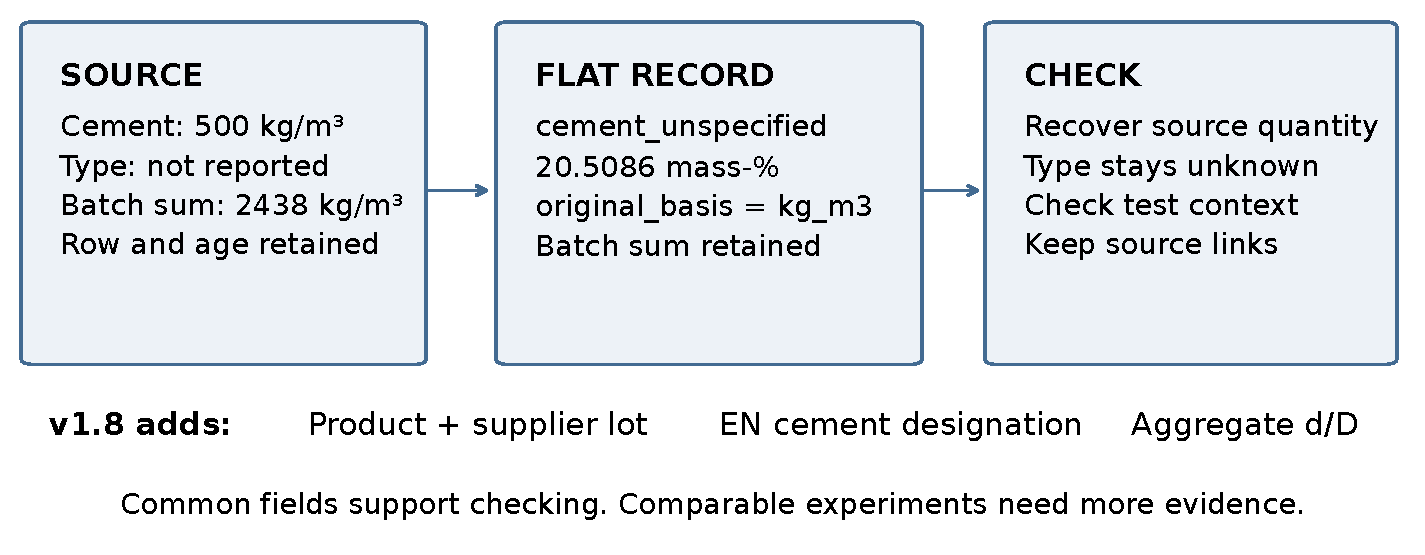
\includegraphics[width=6.4in,height=\textheight,keepaspectratio,alt={Graphical abstract. Keep the source quantity, its meaning and its context together. The 500 kg/m³ cement example comes from the first retained UCI row; its cement classification was not supplied. The product, cement-designation and grading blocks summarize implemented v1.8 additions. This is a reporting schematic, not a physical test or a prediction.}]{figures-v1.2/graphical_abstract.pdf}
\caption{Graphical abstract. Keep the source quantity, its meaning and
its context together. The 500 kg/m³ cement example comes from the first
retained UCI row; its cement classification was not supplied. The
product, cement-designation and grading blocks summarize implemented
v1.8 additions. This is a reporting schematic, not a physical test or a
prediction.}
\end{figure}

\subsection{1. What must survive when a result becomes a
row?}\label{what-must-survive-when-a-result-becomes-a-row}

The first row in the retained UCI example contains 500 kg/m³ of cement
and a compressive strength of 12.64 MPa at one day. It does not identify
the cement as ASTM C150 Type I. A conversion that places this quantity
in \texttt{cement\_type\_1} adds a classification the source did not
give. The corrected representation uses \texttt{cement\_unspecified},
keeps the mass basis, and leaves the cement classification unresolved
{[}1, 2{]}.

This small example captures the paper's central question: what must a
reporting format keep so that the next reader can understand and check a
result? A number may survive copying while its meaning changes.
Kilograms per cubic metre can become percent of binder; a supplier
strength class can become a measured concrete strength; a group mean can
become an apparent specimen result. Each error can produce a
plausible-looking table.

Extrusion printing adds further context. Pumping, deposition, layer
timing and curing affect the state of the material being tested.
Rheological requirements and interlayer behaviour have established
research literatures {[}3--5{]}. Recording these conditions is useful
even when the intended analysis uses only a few of them. Their presence
does not make unlike tests comparable; it helps a reader identify the
differences before combining results.

Open3DCP is a schema specification, maintained as a column reference,
SQL definition and supporting mappings {[}1{]}. It is not a specimen
database service. The repository includes small licensed conversion
examples, but those examples do not make the specification a research
dataset. The format requires no particular printer, supplier,
formulation engine or commercial software. Researchers can use the
relevant columns in ordinary tabular tools and retain detailed source
records alongside them.

This paper makes three contributions: it explains the consequential
recording choices; documents the maintained v1.8 changes against the
v1.7.5 snapshot described in manuscript v1.1; and checks the retained
examples closely enough to distinguish successful arithmetic from
unsupported interpretation. No new mix was produced, no model was
trained, and no construction performance was qualified for this
revision.

\subsubsection{1.1 Scope and version
boundary}\label{scope-and-version-boundary}

The maintained project scope is extrusion-based 3D concrete printing and
hydraulic cementitious systems, including Portland and blended cements,
calcium-aluminate and calcium-sulfoaluminate cements, and high-calcium
alkali-activated slag. Low-calcium fly-ash geopolymer systems and
particle-bed, binder-jetting, spray and slip-form processes remain
outside the project's stated scope {[}1{]}. This is a scope decision,
not a claim that those materials or processes cannot be represented
digitally. The existing activator fields do not establish complete
coverage of every alkali-activated chemistry.

The word \emph{standard} in the project name identifies an open
reporting proposal. Open3DCP is not endorsed or certified by ASTM, CEN,
ACI, ICC, ISO or RILEM. Referenced standards govern their own material
definitions and test procedures. The schema stores descriptions and
results; it does not replace the underlying procedures or professional
decisions.

Schema and manuscript versions are separate. This manuscript is a v1.2
preprint revision. Its technical target is the maintained v1.8 draft at
the full commit identified in Appendix A. The changelog labels that
schema increment 1.8.0. Public availability of the draft does not imply
formal ratification or a matching Zenodo deposit. The concept DOI
identifies the schema series, not this manuscript.

\subsection{2. A source record before and after
conversion}\label{a-source-record-before-and-after-conversion}

Table 1 uses the first data row in the frozen UCI excerpt. Row numbers
here exclude the CSV header and identify this excerpt, not a claimed
original UCI specimen identifier. The source supplies seven constituent
masses, age and strength. It supplies neither a cement standard
designation nor aggregate grading. The conversion should not infer these
properties from what is common in concrete practice.

\begin{longtable}[]{@{}
  >{\raggedright\arraybackslash}p{(\linewidth - 4\tabcolsep) * \real{0.3333}}
  >{\raggedright\arraybackslash}p{(\linewidth - 4\tabcolsep) * \real{0.3333}}
  >{\raggedright\arraybackslash}p{(\linewidth - 4\tabcolsep) * \real{0.3333}}@{}}
\caption{Source-to-field example. Quantities in the first column are
source values; the constituent fields store the mass-percent projection,
calculated in Section 4.1. The schema count is not a requirement to fill
every field.}\tabularnewline
\toprule\noalign{}
\begin{minipage}[b]{\linewidth}\raggedright
Source statement
\end{minipage} & \begin{minipage}[b]{\linewidth}\raggedright
Recorded representation
\end{minipage} & \begin{minipage}[b]{\linewidth}\raggedright
Information still missing
\end{minipage} \\
\midrule\noalign{}
\endfirsthead
\toprule\noalign{}
\begin{minipage}[b]{\linewidth}\raggedright
Source statement
\end{minipage} & \begin{minipage}[b]{\linewidth}\raggedright
Recorded representation
\end{minipage} & \begin{minipage}[b]{\linewidth}\raggedright
Information still missing
\end{minipage} \\
\midrule\noalign{}
\endhead
\bottomrule\noalign{}
\endlastfoot
Cement: 500 kg/m³ & \texttt{cement\_unspecified}; preserve source mass
and basis & ASTM/EN type and supplier designation \\
Fine aggregate: 613 kg/m³ & \texttt{fine\_agg\_unspecified} & Fineness
modulus and grading \\
Coarse aggregate: 1125 kg/m³ & \texttt{coarse\_agg\_unspecified} & Size
designation and grading \\
Water: 200 kg/m³ & \texttt{water}, projected on the declared wet-mass
basis & Aggregate moisture correction, if any \\
Slag, fly ash and superplasticizer: zero & Explicit zeros in those
fields & No positive dosage inferred \\
Strength: 12.64 MPa at one day & Strength and age retained separately &
Specimen geometry and detailed test procedure \\
\end{longtable}

The generic constituent fields were already implemented in v1.7.5. They
are not new v1.8 additions. Their purpose is to keep a stated quantity
without inventing a more specific class. Similarly,
\texttt{admixture\_basis=as\_delivered} records the basis of a delivered
product when its solids fraction is unknown. A missing solids fraction
must not be silently replaced by an assumed percentage.

\texttt{NULL} means the value is unavailable for the record. It can mean
unreported, unknown, unmeasured or inapplicable. These reasons are not
identical, and the single null value does not encode their distinction.
When the reason matters, record it in the provenance notes or a linked
curation record. Zero is appropriate only when the source reports zero
or absence. Blank constituent cells in a proprietary premix do not mean
the product contains none of those constituents.

The distinction between unspecified and other is also deliberate.
\texttt{cement\_unspecified} is for an unknown type. In v1.8,
\texttt{cement\_other} is for a stated type that has no dedicated
quantity column; its exact designation belongs in
\texttt{cement\_designation}. A curator should not turn a known but
unsupported designation into an unknown one merely to fit the
vocabulary.

\subsection{3. What one Open3DCP record
represents}\label{what-one-open3dcp-record-represents}

\subsubsection{3.1 A flat core with linked
detail}\label{a-flat-core-with-linked-detail}

The SQL implementation calls its main table \texttt{mix\_designs}. It
has an internal \texttt{id}, a unique required \texttt{mix\_id}, a
required \texttt{name}, optional parent and batch labels, and fields for
composition, process, tests, properties and provenance. Its practical
core is a formulation-centred record with selected context and scalar
results. It is not a fully normalized specimen, event and test database
{[}1{]}.

This matters because the examples have different row meanings. UCI rows
describe mix-and-age observations. Meta rows describe reported
mix-and-age summaries. RILEM rows are aggregates assembled by an
extraction script. The UF excerpt carries selected age-specific results
from literature records. The buildings example describes projects. They
must not all be described as one specimen per row.

For an analytical export, the curator needs to state what each row
represents and preserve a source key. If several tests or batches share
a formulation, their relationship must remain available in the source
tables or an explicit sidecar. A \texttt{parent\_mix\_id} can document a
variant relationship, but in the frozen DDL it is text, not an enforced
foreign key. Likewise, \texttt{batch\_label} identifies a local batch
context; it is not a normalized batch table.

\begin{figure}
\centering
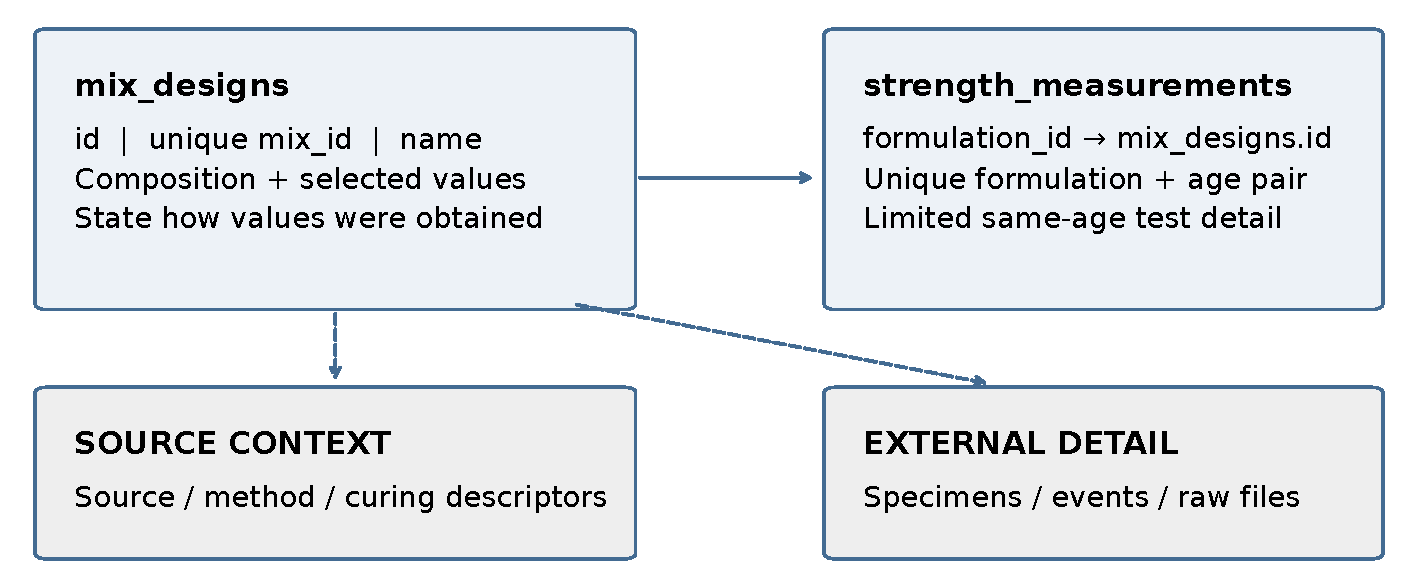
\includegraphics[width=6.3in,height=\textheight,keepaspectratio,alt={Relationship view of the maintained SQL. The main record supports a convenient flat view. Age-specific results link through formulation\_id; raw files and source detail remain external where the scalar row cannot carry them. Dashed connections indicate descriptive references, not additional enforced SQL foreign keys.}]{figures-v1.2/record_relationships.pdf}
\caption{Relationship view of the maintained SQL. The main record
supports a convenient flat view. Age-specific results link through
\protect\texttt{formulation\_id}; raw files and source detail remain
external where the scalar row cannot carry them. Dashed connections
indicate descriptive references, not additional enforced SQL foreign
keys.}
\end{figure}

\subsubsection{3.2 Companion-table limits}\label{companion-table-limits}

The maintained DDL creates \texttt{strength\_measurements},
\texttt{sources}, \texttt{test\_methods}, \texttt{curing\_regimes} and
\texttt{standard\_test\_ages} in addition to \texttt{mix\_designs}. The
first of these references \texttt{mix\_designs(id)} through
\texttt{formulation\_id}. It also imposes
\texttt{UNIQUE(formulation\_id,\ test\_age\_days)}. This is useful for
one age-series record per formulation and age, but cannot separately
hold every replicate, orientation and test method at the same age under
that same key.

Consequently, the companion table does not solve all specimen-level
relationships. A claim that the format preserves the full experimental
chain without joins is too strong. The schema can hold selected values
and references; detailed geometry, print events, replicate identities,
test histories and files may still need their original relational
representation. This paper documents that boundary rather than changing
the schema to resolve it.

The example CSVs also lack the required SQL identity columns. They are
partial tabular excerpts, not ready-to-insert database instances. The
buildings file includes ten project columns outside the main vocabulary;
UF adds \texttt{source\_dataset}. Their descriptive value remains, but
their filenames do not establish strict conformance to the canonical
main table. The companion audit lists these fields explicitly.

\subsubsection{3.3 Measured, derived and aggregated
values}\label{measured-derived-and-aggregated-values}

A source measurement, a unit conversion, a calculated ratio and a group
mean are different operations. A row-level
\texttt{measurement\_confidence} flag is too coarse to explain all of
them in a mixed record. Use the source reference and curation ledger to
identify which values were reported, converted or aggregated, and retain
the input values for derived quantities.

A standard deviation needs its definition, sample count and grouping
rule. Population standard deviation uses a divisor of \(n\); sample
standard deviation uses \(n-1\). Neither is automatically a standard
error, and neither resolves dependence among specimens from one print or
batch. The old RILEM excerpt stored calculated group summaries while
labelling the record measured. That label did not describe the
extraction sufficiently.

\subsection{4. Recording quantities without changing their
meaning}\label{recording-quantities-without-changing-their-meaning}

\subsubsection{4.1 The mass-basis bridge}\label{the-mass-basis-bridge}

The maintained contract treats source kg/m³ as the primary practical
reporting basis and stores constituent columns as mass-percent of total
wet mix. \texttt{original\_basis} identifies the incoming basis.
\texttt{total\_batched\_mass\_kg\_m3} is the sum used in the projection,
while \texttt{total\_binder\_kg\_m3} retains the cementitious total for
binder-relative calculations. The batched-mass total is not a measured
fresh density.

Let \(m_i\) be the reported mass of constituent \(i\) on the common
kg/m³ basis, and let \(M=\sum_i m_i\). For a complete, consistently
accounted inventory with \(M>0\),

\[p_i=100\frac{m_i}{M},\qquad m_i=\frac{p_iM}{100}. \tag{1}\]

No measured density enters these equations. They preserve the reported
proportional basis even if the source's design quantities do not
demonstrably yield exactly one physical cubic metre. A yield discrepancy
is still a discrepancy and must travel with any per-volume
interpretation.

For the UCI row in Section 2, \(M=500+200+1125+613=2438\) kg/m³ and the
reported binder total is 500 kg/m³. Table 2 shows the calculation. The
display rounds percentages to four decimal places; the evidence file
retains the full stored values.

\begin{longtable}[]{@{}
  >{\raggedright\arraybackslash}p{(\linewidth - 6\tabcolsep) * \real{0.2500}}
  >{\raggedleft\arraybackslash}p{(\linewidth - 6\tabcolsep) * \real{0.2500}}
  >{\raggedleft\arraybackslash}p{(\linewidth - 6\tabcolsep) * \real{0.2500}}
  >{\raggedleft\arraybackslash}p{(\linewidth - 6\tabcolsep) * \real{0.2500}}@{}}
\caption{A worked round trip on a real retained row. Display rounding
explains the small differences. The full-precision reconstruction is
checked separately.}\tabularnewline
\toprule\noalign{}
\begin{minipage}[b]{\linewidth}\raggedright
Constituent
\end{minipage} & \begin{minipage}[b]{\linewidth}\raggedleft
Source kg/m³
\end{minipage} & \begin{minipage}[b]{\linewidth}\raggedleft
Mass-percent
\end{minipage} & \begin{minipage}[b]{\linewidth}\raggedleft
Recovered kg/m³ from displayed percent
\end{minipage} \\
\midrule\noalign{}
\endfirsthead
\toprule\noalign{}
\begin{minipage}[b]{\linewidth}\raggedright
Constituent
\end{minipage} & \begin{minipage}[b]{\linewidth}\raggedleft
Source kg/m³
\end{minipage} & \begin{minipage}[b]{\linewidth}\raggedleft
Mass-percent
\end{minipage} & \begin{minipage}[b]{\linewidth}\raggedleft
Recovered kg/m³ from displayed percent
\end{minipage} \\
\midrule\noalign{}
\endhead
\bottomrule\noalign{}
\endlastfoot
Unspecified cement & 500.0 & 20.5086 & 499.999668 \\
Water & 200.0 & 8.2034 & 199.998892 \\
Unspecified coarse aggregate & 1125.0 & 46.1444 & 1125.000472 \\
Unspecified fine aggregate & 613.0 & 25.1436 & 613.000968 \\
Slag, fly ash, superplasticizer & 0.0 each & 0.0000 each & 0.000000
each \\
\end{longtable}

The read-only check reconstructs all 98 constituent cells in the 14-row
UCI excerpt from the stored percentages and batch totals. The largest
floating-point difference is \(2.28\times10^{-13}\) kg/m³, rounded
upward. Rounding all percentages to four decimal places increases the
largest error across that excerpt to about 0.00123 kg/m³. These are
arithmetic checks on the stated inventory, not uncertainty estimates for
the underlying measurements.

The conditions are essential. Include each constituent once, on a
consistent wet/as-delivered or solids-plus-carrier basis. Do not count a
solution both as a whole and as its separated components. Do not
normalize a partially reported inventory and call it total-mix
composition. Preserve the source precision and document any conversion
input. A volume dosage needs the appropriate density to become mass; a
mass inventory already reported on a common basis does not.

\subsubsection{4.2 Ratios, water and
admixtures}\label{ratios-water-and-admixtures}

Absolute binder dosage is necessary to recover kg/m³ from
binder-relative ratios, but is not necessary to recover mass fractions
from a complete set of mass ratios. If \(r_i=m_i/B\) for a common binder
reference \(B\), then

\[p_i=100\frac{r_i}{\sum_j r_j}. \tag{2}\]

The scale \(B\) cancels. Ratios expressed as percent of binder first
require division by 100. A binder total must not be counted again
alongside all of its component ratios. This corrects the earlier paper's
explanation of the UF example. Section 6 describes the remaining
source-specific ambiguities; the revision does not fabricate missing
quantities to complete that inventory.

The water-to-binder ratio also needs an accounting definition. The
maintained convention uses the recorded water column relative to
cementitious material. Carrier water inside an as-delivered admixture is
not automatically added. Thus a computed \texttt{w\_b\_ratio} may differ
from an effective-water ratio that includes aggregate moisture,
absorption or admixture carrier water. Keep the stated ratio and its
definition visible when those inputs are unavailable. Do not use a
dry-product bulk density as a substitute for wet-mix density or batch
yield.

\subsubsection{4.3 Units and conversion
checks}\label{units-and-conversion-checks}

Strength columns use MPa, elastic modulus uses GPa, and rheological
stresses use Pa. A column name helps the reader, but does not prevent
incorrect input. The v1.8 \texttt{crosswalk/units.csv} records units,
quantity kinds and conversion factors for a consistent
mm--N--tonne--second finite-element unit system. For example, MPa equals
N/mm², while kg/m³ converts to tonne/mm³ by multiplying by \(10^{-12}\)
{[}1{]}.

This file is a unit mapping, not a finite-element material model. A
blank factor must not be treated as one. In particular,
\texttt{cement\_strength\_class\_mpa} is a classification and
deliberately has no physical stress conversion. Export still needs a
choice of constitutive model, applicable test data and engineering
interpretation. The existence of a unit manifest does not establish a
validated solver integration.

\subsection{5. What changed in the maintained v1.8
draft?}\label{what-changed-in-the-maintained-v1.8-draft}

The frozen SQL comparison finds 31 added main-table fields and no
removed fields. Excluding \texttt{id}, the count rises from 248 to 279.
Including it, the counts are 249 and 280. The previous categorical
growth figures are replaced by this direct comparison; no claim that
schema growth has stabilized is retained. Appendix A groups the
additions, and the evidence package lists every column and SQL
definition.

\subsubsection{5.1 Commercial premix
identity}\label{commercial-premix-identity}

Six fields record \texttt{is\_premixed}, \texttt{supplier},
\texttt{product\_name}, \texttt{supplier\_batch\_number},
\texttt{production\_date} and \texttt{bulk\_density\_kg\_m3}. They allow
a record to identify a purchased material even when its constituent
recipe is proprietary. \texttt{supplier\_batch\_number} is the
supplier's lot; \texttt{batch\_label} remains the user's local
repeat-batch identifier. \texttt{production\_date} concerns manufacture
of the supplied material, while \texttt{date\_of\_casting} concerns the
concrete batch and curing clock.

Product and lot identity improve traceability. They do not, by
themselves, make a print reproducible. Water addition, storage
condition, mixing, process settings, curing and test context still
matter. An undisclosed recipe can remain unknown while the available
product evidence is recorded accurately. The revised paper therefore
does not repeat the changelog's stronger suggestion that these fields
fully determine reproducibility.

\subsubsection{5.2 Cement designations must remain
distinct}\label{cement-designations-must-remain-distinct}

The v1.8 draft introduces 18 EN cement quantity columns. Four keep the
limestone distinctions explicit: \texttt{cem\_ii\_a\_l},
\texttt{cem\_ii\_a\_ll}, \texttt{cem\_ii\_b\_l} and
\texttt{cem\_ii\_b\_ll}. They must not collapse into
\texttt{cement\_type\_1l}. In v1.8, \textbf{\texttt{cement\_type\_1l}
means ASTM C595 Type IL only}. Type IL is written with a capital I and L
in the standard designation; the existing schema identifier uses the
digit 1 {[}1, 6{]}.

Preserve the exact source designation in \texttt{cement\_designation}.
\texttt{cement\_standard} identifies its designation system. The numeric
supplier class belongs in \texttt{cement\_strength\_class\_mpa}. The L,
N or R designation belongs in \texttt{cement\_early\_strength\_class}. A
designation such as CEM I 42.5 R is a cement classification, not a
measured 42.5 MPa result for the printed mix. Nor does R alone quantify
the open time or buildability of a formulation. These fields should not
be derived from concrete strength tests.

The new \texttt{cement\_other} field retains a stated hydraulic-cement
type outside the dedicated columns. Together, a quantity field, verbatim
designation and designation system are more informative than either a
forced ASTM approximation or an isolated free-text note. They remain a
record of the source claim: entering a standard designation does not
prove that a material satisfies that standard.

\subsubsection{5.3 Aggregate size
fractions}\label{aggregate-size-fractions}

\texttt{agg\_fraction\_d\_lower\_mm} and
\texttt{agg\_fraction\_d\_upper\_mm} retain the lower and upper sizes of
a stated aggregate fraction when that is the information available.
These fields complement the existing fineness-modulus approach. A size
interval alone does not determine the sieve distribution and cannot
yield a fineness modulus. Neither a size interval nor fineness modulus
alone certifies aggregate grading compliance.

The paper's former statement that 3DCP uses only fine aggregate is
withdrawn. Equipment and application constrain aggregate selection; the
schema already includes coarse-aggregate fields. The useful reporting
principle is to preserve the grading evidence actually supplied, without
inventing a distribution to populate a preferred field.

\subsubsection{5.4 Compatibility and
extensions}\label{compatibility-and-extensions}

The DDL additions are structurally additive, but the cement mapping
requires semantic care. Pre-v1.8 \texttt{cement\_type\_1l} rows may mean
ASTM Type IL or EN CEM II/A-L under the former dual mapping. An old
header alone cannot distinguish them. Retain the old schema version and
inspect the source designation before reclassification. This manuscript
does not migrate any records.

The maintained draft reserves \texttt{x\_} for documented site-specific
extension columns. That reservation does not turn such fields into
canonical Open3DCP columns. Gaps should be proposed upstream with their
type, unit, reporting basis, range and primary technical reference. A
local export or a paper revision must not silently redesign the shared
schema.

\subsubsection{5.5 The existing material and test
vocabulary}\label{the-existing-material-and-test-vocabulary}

The additions sit within a broader reporting vocabulary. The binder and
supplementary-material fields distinguish stated material families;
aggregate, fiber, admixture, pigment and activator fields retain
quantities alongside descriptors. These are separate ingredients and
attributes, not a claim that all fields should be used together. A
purchased blended cement should not be counted once as a cement and
again as inferred clinker and additions unless a clearly documented
decomposition replaces the original quantity.

Fiber dosage and geometry are recorded separately.
\texttt{fiber\_length\_mm}, \texttt{fiber\_diameter\_mm} and
\texttt{fiber\_aspect\_ratio} describe different attributes; calculating
their ratio requires compatible units and a meaningful common fiber
population. A single length or diameter cannot describe a multimodal
fiber mixture. The scalar summary should therefore retain its population
definition in the source context, with distributions kept externally
where available.

Fresh-state fields include static and dynamic yield stress, plastic
viscosity, structuration rate, spread, setting times and other
workability measurements. These quantities are not interchangeable tests
of printability. A recorded \texttt{static\_yield\_stress\_pa} requires
the measurement time, apparatus and loading history to be interpretable.
\texttt{structuration\_rate\_pa\_per\_s} records a rate, not a yield
stress. \texttt{rheology\_curve\_file} can point to the underlying
curve, while a scalar field carries the reported summary {[}1, 3{]}.

Process fields cover print speed, nozzle geometry, layer dimensions,
extrusion rate, mixing and pumping. In particular,
\texttt{layer\_time\_gap\_s} denotes a local interval between layers at
a point. A total job duration or travel time for a whole object is not
automatically that interval. A single nominal value is useful only with
a statement of the print schedule it summarizes. The original machine
log can retain variation that the scalar field omits.

Mechanical fields include compressive, tensile, flexural and bond
strengths, modulus, toughness and related quantities.
\texttt{interlayer\_bond\_mpa} and \texttt{interlayer\_shear\_mpa} are
dedicated interface fields; a general bond result must not be relabelled
interlayer merely because the specimen was printed. Test method,
specimen preparation, orientation and failure location still determine
the meaning of the result. The available uncertainty fields support
selected summaries, not a complete uncertainty budget for every column.

The durability and thermal vocabulary goes beyond strength. The charge
result is recorded in \texttt{chloride\_rcpt\_coulombs}. The chloride
migration and diffusion fields represent coefficients. Their numerical
values must not be interchanged or combined under a generic
chloride-resistance label. Exposure descriptions and test-method
references help identify the intended interpretation; they do not
convert an accelerated test into an established service-life prediction
{[}1{]}.

Finally, \texttt{raw\_data\_doi}, \texttt{stress\_strain\_file},
\texttt{microstructure\_image} and \texttt{raw\_data\_file} preserve
references to larger evidence. A resolvable file, its units, license and
sample linkage remain the depositor's responsibility. A filename alone
cannot reconstruct the acquisition method. These existing fields support
the composition-process-condition-property-provenance chain while
keeping its incomplete parts visible.

\subsection{6. What the five retained examples
demonstrate}\label{what-the-five-retained-examples-demonstrate}

\subsubsection{6.1 Scope of the evidence}\label{scope-of-the-evidence}

The frozen examples contain 71 rows: 14 UCI, 28 Meta, 9 RILEM, 10 UF and
10 buildings. Selection was purposive, not random. The sources exercise
different reporting situations and have different observational units. A
row count is therefore a description of the artifacts, not a sample size
for a pooled scientific conclusion.

\begin{longtable}[]{@{}
  >{\raggedright\arraybackslash}p{(\linewidth - 6\tabcolsep) * \real{0.2500}}
  >{\raggedleft\arraybackslash}p{(\linewidth - 6\tabcolsep) * \real{0.2500}}
  >{\raggedright\arraybackslash}p{(\linewidth - 6\tabcolsep) * \real{0.2500}}
  >{\raggedright\arraybackslash}p{(\linewidth - 6\tabcolsep) * \real{0.2500}}@{}}
\caption{Evidence coverage. These excerpts do not establish adoption at
scale, predictive performance or physical validation. Dataset-level
attribution is retained in each example's source and notice
files.}\tabularnewline
\toprule\noalign{}
\begin{minipage}[b]{\linewidth}\raggedright
Source
\end{minipage} & \begin{minipage}[b]{\linewidth}\raggedleft
Retained rows
\end{minipage} & \begin{minipage}[b]{\linewidth}\raggedright
Selection and row meaning
\end{minipage} & \begin{minipage}[b]{\linewidth}\raggedright
Demonstrated use and limit
\end{minipage} \\
\midrule\noalign{}
\endfirsthead
\toprule\noalign{}
\begin{minipage}[b]{\linewidth}\raggedright
Source
\end{minipage} & \begin{minipage}[b]{\linewidth}\raggedleft
Retained rows
\end{minipage} & \begin{minipage}[b]{\linewidth}\raggedright
Selection and row meaning
\end{minipage} & \begin{minipage}[b]{\linewidth}\raggedright
Demonstrated use and limit
\end{minipage} \\
\midrule\noalign{}
\endhead
\bottomrule\noalign{}
\endlastfoot
UCI/Yeh {[}2{]} & 14 & Curated mix-and-age rows spanning composition and
age & Mass projection; cement and grading remain unspecified \\
Meta SustainableConcrete {[}7{]} & 28 & Six selected mixes across
reported ages & Quantity, strength-summary and GWP fields; no printing
evidence \\
RILEM ILS-mech {[}8{]} & 9 & Selected aggregates for mixes 01\_a, 13\_a,
19\_a & Source linkage and grouping audit; earlier effect claim
withdrawn \\
UF mix-design compilation {[}9{]} & 10 & Selected literature rows with
rheology, w/b and strength & Unit conversion and source context; ratio
accounting unresolved \\
Buildings catalogue {[}10{]} & 10 & Fixed project IDs across selected
buildings & Project metadata; ten project columns are outside the main
schema \\
\end{longtable}

The UCI source has nine numeric columns. The retained Meta input adds
uncertainty summaries and GWP values. Those are distinct data
attributes, not evidence that the two sources use interchangeable tests.
The buildings script selects source IDs 12, 18, 20, 45, 47, 50, 63, 64,
67 and 58; it does not extract material performance. The earlier
surveyed UHPC coded matrix remains excluded from the demonstration
because its usable mapping was not established. No new assessment of
that source's access conditions is claimed here.

\subsubsection{6.2 RILEM: the earlier grouping does mix incompatible
contexts}\label{rilem-the-earlier-grouping-does-mix-incompatible-contexts}

The previous paper reported flexural reductions of 32--55\% relative to
cast reference groups. The review initially established missing
safeguards in the extraction code, not actual contamination. The present
read-only audit goes further: it inspects the original SQLite export and
matches the nine retained rows to their raw aggregate means and counts.

The legacy query selects three mix-name prefixes, accepts numeric
strengths at ages 20--40 days, and groups by compound orientation. It
does not separate test method, scale or default/deviating conditions.
The raw data confirm these distinctions are present inside the selected
groups. For example, the 01\_a cast group includes both three- and
four-point bending and both mortar- and concrete-scale specimens. The
01\_a U.W group includes both bending methods, ages 28 and 29 days, and
DEFAULT plus DEV1 conditions. The corresponding 13\_a U.W group includes
DEFAULT, DEV1 and DEV2. The 19\_a cast and U.W groups also combine
bending methods.

These are observations about the audited extraction, not a criticism of
the RILEM experiment. Its study plan explicitly distinguishes these
cases. The primary analysis separates test type, scale and process
condition, and applies its own age and outlier criteria {[}11, 12{]}.
The old excerpt did not reproduce that analysis.

All nine retained means and counts match raw legacy aggregates to their
published precision. That confirms where the numbers came from; it does
not validate the comparisons. Moreover, the current legacy script would
enumerate 12 orientation groups from this database, while only nine are
retained. The omitted groups are 01\_a V.U, 13\_a W.U and 19\_a W.U. No
documented selection rationale for those omissions was found in the
inspected script and source note.

The 32--55\% conclusion and its error interpretation are withdrawn from
the abstract, results and figure. This revision does not substitute a
new effect estimate. A defensible reanalysis would need source-linked
print and batch identities, matched methods and scales, explicit age and
condition rules, and an uncertainty treatment that respects clustering.
The accompanying inclusion ledger preserves the individual source codes
and context so that this work can be reviewed independently.

\subsubsection{6.3 Orientation needs the full test
geometry}\label{orientation-needs-the-full-test-geometry}

The old mapping used the first part of compound RILEM codes to create
X/Y/Z labels. That projection is insufficient for flexure. Force
direction, beam axis and tensile-stress direction are different
geometric quantities. The original compound code must remain available
in source-linked notes or a sidecar even when a simpler analytical field
is also used.

\begin{figure}
\centering
\includegraphics[width=6.2in,height=\textheight,keepaspectratio,alt={Orientation schematic for reading a flexural record. Print-path direction U, transverse direction V and build direction W define the material frame. A flexural record also needs the beam axis, applied force and tensile-stress direction. The illustrated U.W case places tensile stress normal to layer interfaces; it is not a universal X/Y/Z strength ordering. Geometry is schematic and follows the source study's orientation discussion {[}11, 12{]}.}]{figures-v1.2/orientation.pdf}
\caption{Orientation schematic for reading a flexural record. Print-path
direction U, transverse direction V and build direction W define the
material frame. A flexural record also needs the beam axis, applied
force and tensile-stress direction. The illustrated U.W case places
tensile stress normal to layer interfaces; it is not a universal X/Y/Z
strength ordering. Geometry is schematic and follows the source study's
orientation discussion {[}11, 12{]}.}
\end{figure}

The revised paper removes the earlier highest/moderate/lowest strength
table. A source-defined coordinate system and test diagram are more
useful than a universal ranking. Keep CAST as the recorded reference
preparation; do not treat it as proof that all cast specimens are
isotropic or that every cast and printed pair is otherwise matched.

\subsubsection{6.4 UF: correct the reason for leaving composition
unresolved}\label{uf-correct-the-reason-for-leaving-composition-unresolved}

The original workbook was inspected read-only. Applying the script's
selection order finds ten source rows and ten age-specific outputs. It
selects rows with numeric static yield stress, water/binder ratio and at
least one strength value, with at most two rows per reference. The code
does not actually apply the explicit printable-Portland filter described
in its introductory comment.

The workbook contains useful binder-relative quantities. For example,
source spreadsheet row 46 states cement, fly ash and silica-fume ratios
of 0.47, 0.47 and 0.06, with water/binder 0.30 and sand/binder 0.50. If
these were the complete constituent inventory, Equation 2 would
normalize them without an absolute binder dosage. Blank admixture
entries, however, are not explicit zero evidence.

Other selected rows contain admixture or activator descriptors beneath
mixed percent-of-binder and ratio headers. The extractor also probes
some constituent-name cells as numbers when identifying supplementary
materials. The current excerpt's chemistry labels therefore require
further curation. This revision retains the example as a reporting
audit, corrects the false mathematical explanation, and leaves
composition unconverted pending complete source accounting. No unknown
density or binder dosage is invented.

\subsubsection{6.5 Carbon records are not a strength--carbon
result}\label{carbon-records-are-not-a-strengthcarbon-result}

The Meta excerpt records reported GWP and strength summaries at stated
ages. The source repository separates measured data from model proposals
{[}7{]}. This is useful provenance, but does not establish a general
relationship between binder carbon and concrete strength. The earlier
highlighted pair mixed composition and water/binder effects and carried
a yield caveat.

This revision removes the pairwise carbon-reduction headline. Retaining
it as a result would require a matched account of source row IDs,
measured versus generated status, test age and method, GWP boundary and
factors, and the per-volume yield basis. The retained example continues
to demonstrate fields for those reported quantities. It does not
demonstrate that Open3DCP reduces carbon or that a low-clinker
formulation meets a structural requirement.

\subsection{7. What the conversion checks
establish}\label{what-the-conversion-checks-establish}

\subsubsection{7.1 Counts before scores}\label{counts-before-scores}

The retained UCI fidelity report counts 126 routed cells, corresponding
to 14 rows and nine source fields. It separately scores 117 substantive
value cells and marks 47 as generically recorded. Its 100/A grade
reflects the applicable dimensions under the maintainer's scoring rules.
These denominators are not all counts of independent measurements.

The retained Meta report counts 516 populated source fields, of which 48
selector/metadata fields are excluded from the field-coverage
denominator. It reports 468 mapped fields, 459 substantive value cells
and 103 generic cells. Coverage is 100\% on its chosen denominator and
about 91\% across all 516 populated fields. These figures describe the
retained tool report, not an independently calibrated quality scale.

A score cannot detect an error that the rules do not test. In
particular, generic storage can preserve a quantity while leaving its
scientific classification unresolved. Source selection, incorrect
grouping, implicit basis assumptions and missing relationships need
separate review. A high grade is not evidence of physical validation,
interoperability with every consumer or suitability for model training.

\subsubsection{7.2 Structural checks and scientific checks
differ}\label{structural-checks-and-scientific-checks-differ}

Four maintained checks were executed on the frozen v1.8 snapshot:
version consistency, public schema-reference consistency, generated
precedent-crosswalk consistency and units-manifest consistency. All
passed. The UCI arithmetic round trip was also executed. These checks
support the stated version, vocabulary and conversion arithmetic. They
do not establish correctness of every source mapping or every
material-science description.

The SQL supplies types, identity constraints and the age-table
relationship described earlier. Most scientific ranges and vocabularies
are documentary conventions rather than SQL \texttt{CHECK} constraints.
Even the submission validator is a metadata checklist, not a
specimen-level scientific validator; its frozen version warning still
refers to schema 1.6. This is recorded as a maintenance issue rather
than silently corrected in a manuscript task.

Before analytical reuse, a curator should verify the source key,
reporting basis, units, missingness, material designation, test context
and row meaning. A mechanical comparison additionally needs matching
specimen geometry, preparation, age, orientation and condition. A
computed summary needs the exact inclusion set and statistic. These are
review requirements for the intended analysis, not a new claim that the
current software enforces them all.

\subsubsection{7.3 Reproducibility and model
use}\label{reproducibility-and-model-use}

The package freezes input hashes, the schema commit, audit scripts and
figure inputs. Each revised figure has editable generation code. The
column counts are checked against the generated inventory; the figures
are explanatory schematics rather than statistical plots. The original
source database and publication editions are unchanged.

For machine learning, grouping choices should precede train/test
splitting. Specimens from one batch, repeated ages of one mix, and
aggregates from one source can be dependent. A random row split can
place related observations in both training and evaluation sets.
Source-aware and formulation-aware evaluation is needed for the
particular prediction question. Design strength can leak a target, and
derived ratios and the two mass bases carry overlapping information.
These risks are not resolved by a common column vocabulary.

\subsection{8. How the format relates to other data
models}\label{how-the-format-relates-to-other-data-models}

The closest comparison is the RILEM database: it preserves entities and
relationships needed for its interlaboratory study {[}8, 13{]}. Its
existing analyses show that cross-laboratory comparison did not become
possible only with Open3DCP. A flat export can make selected quantities
easier to inspect, while the original database remains necessary for
relationships and context that the export omits.

AM-CDM, GEMD and CPTO address related representation needs {[}14--16{]}.
The maintained repository includes model-level mappings to AM-CDM commit
\texttt{141030b}, GEMD format v0.1 and CPTO v1.0.1. These pins describe
the targets used by the mappings, not the latest state of each project.
They allow review at a known boundary without making claims about what
all other models lack.

The mapping files distinguish direct, normalized, derived, partial and
unmapped cases. A field-level correspondence is a proposed
representation relationship; it is not an executed round-trip exchange
test. A graph can preserve relationships that a scalar export omits. A
flat table can be convenient for inspection and analysis. Neither
convenience nor graph structure alone establishes scientific
comparability.

The earlier historical claim that a metal-powder standard ended ad hoc
data reporting is removed. It was not needed to explain Open3DCP.
Likewise, the revised paper makes no exhaustive novelty claim and no
measured curation-time claim. The useful question is whether another
researcher can reconstruct the stated conversion from the source and the
mapping.

Open licensing, persistent references, explicit units and provenance can
support FAIR data practice {[}17{]}. Actual findability, accessibility,
interoperability and reuse depend on the deposited dataset, metadata,
licenses, identifiers and maintained access. The presence of a DOI field
and an open schema is not a FAIR certification.

\subsection{9. What remains outside the record, and how to try
it}\label{what-remains-outside-the-record-and-how-to-try-it}

\subsubsection{9.1 Measurement and representation
gaps}\label{measurement-and-representation-gaps}

The original paper treated several difficult measurements as impossible.
The revised distinction is practical: what was recorded, what could be
measured with limitations, and what the schema can represent. A missing
column does not prove an instrument is unavailable, and an available
research instrument does not establish routine production use.

\begin{longtable}[]{@{}
  >{\raggedright\arraybackslash}p{(\linewidth - 4\tabcolsep) * \real{0.3333}}
  >{\raggedright\arraybackslash}p{(\linewidth - 4\tabcolsep) * \real{0.3333}}
  >{\raggedright\arraybackslash}p{(\linewidth - 4\tabcolsep) * \real{0.3333}}@{}}
\caption{Practical recording gaps. This is a qualitative list, not a
ranked instrumentation roadmap or a claim of unavailable measurement
technology.}\tabularnewline
\toprule\noalign{}
\begin{minipage}[b]{\linewidth}\raggedright
Information
\end{minipage} & \begin{minipage}[b]{\linewidth}\raggedright
Current recording situation
\end{minipage} & \begin{minipage}[b]{\linewidth}\raggedright
Remaining work
\end{minipage} \\
\midrule\noalign{}
\endfirsthead
\toprule\noalign{}
\begin{minipage}[b]{\linewidth}\raggedright
Information
\end{minipage} & \begin{minipage}[b]{\linewidth}\raggedright
Current recording situation
\end{minipage} & \begin{minipage}[b]{\linewidth}\raggedright
Remaining work
\end{minipage} \\
\midrule\noalign{}
\endhead
\bottomrule\noalign{}
\endlastfoot
Point rheology, pump pressure, nominal print settings & Scalar columns
exist & Record timing, apparatus, sampling and relation to deposition \\
Pressure and motion histories; local dosing & A scalar cannot retain an
event history & Keep source logs, clocks, units and event links \\
Material age and changes during printing & Batch dates and notes provide
partial context & Preserve retempering and dosing events without
treating initial composition as the whole print \\
Moisture, temperature and interface condition & Local measurements may
differ from ambient summaries & Record position, time, method and
spatial coverage \\
Fiber orientation and internal pore structure & Imaging can characterize
sampled material & Retain resolution, sample preparation, segmentation
and representativeness \\
Replicate tests and print relationships & Main row and age table have
limited cardinality & Keep original specimen and print records linked \\
\end{longtable}

X-ray computed tomography can image internal structure; sample
preparation, size, contrast, resolution and analysis limit what is
inferred {[}18{]}. Removing a specimen from a larger object may be
destructive even when imaging that specimen is not. No ranking of fiber
aspect ratio as the single strongest predictor of toughness is retained.
Similarly, 28 days is a common reporting age, not a complete criterion
for structural adequacy.

The old estimate that a complete digital twin would require more than
300 parameters is removed. No counting model supported it. Open3DCP can
contribute static records and file references to a larger system. It
does not itself implement a live digital twin, a control loop or a
prediction service.

\subsubsection{9.2 A bounded adoption
method}\label{a-bounded-adoption-method}

Start with one source and one analysis question. Preserve the source
files and their license. Select a schema version, declare the row
meaning and retain stable source identifiers. Map the columns without
inventing classifications. Keep the incoming quantity basis and every
conversion input. Use nulls deliberately and record why important values
are missing.

Next, check the conversion against the source. Reconstruct quantities
where the basis permits it. Inspect out-of-vocabulary fields and retain
them for review. For mechanical data, keep specimen and test context
before comparing strengths. For commercial premixes, keep the product
and lot even when the recipe is unavailable. A documented partial record
is useful if the analysis respects its limits.

Report gaps through the upstream issue and contribution process,
preferably with an ORCID, a concrete source example and a primary
definition for the proposed property. Feedback on ambiguous bases, row
relationships, units and hard-to-map designations is more useful than
filling empty cells speculatively. Substantive schema extensions require
their own review; this manuscript revision introduces none.

\subsubsection{9.3 Conclusion}\label{conclusion}

Open3DCP provides a shared vocabulary for recording extrusion-printing
data, with source quantities and context kept visible. The v1.8
additions improve the representation of purchased materials, EN cement
designations and aggregate fractions. The worked mass conversion is
reproducible under stated conditions. The RILEM audit shows why
reproducible arithmetic is not sufficient: a table can retain its
numbers while combining unlike tests.

The appropriate next step is better source-linked curation and
independent review of the mappings. Adoption at scale, inter-curator
agreement, calibrated fidelity scores and downstream predictive value
remain unestablished. The schema is designed to support that work; it
does not stand in for physical testing or engineering qualification.

\newpage

\subsection{Appendix A. Frozen versions and field
changes}\label{appendix-a.-frozen-versions-and-field-changes}

\textbf{Schema target:}
\texttt{fa5fdd5a513dee4554fd3fc01cab967a9ebd6041}, public main read back
on 15 September 2026. Baseline: schema tag v1.7.5. The isolated task
checkout itself began at
\texttt{af422a27dc24f301ddc8f67d397f3fed58dbc0ed}; it was not mistaken
for current main.

\begin{longtable}[]{@{}
  >{\raggedright\arraybackslash}p{(\linewidth - 4\tabcolsep) * \real{0.3333}}
  >{\raggedright\arraybackslash}p{(\linewidth - 4\tabcolsep) * \real{0.3333}}
  >{\raggedleft\arraybackslash}p{(\linewidth - 4\tabcolsep) * \real{0.3333}}@{}}
\caption{Implemented additions. The accompanying
\protect\texttt{schema\_columns.csv} provides the complete inventory and
SQL types. Ranges and designation details remain in the pinned schema
reference; this table does not replace a material
standard.}\tabularnewline
\toprule\noalign{}
\begin{minipage}[b]{\linewidth}\raggedright
Group
\end{minipage} & \begin{minipage}[b]{\linewidth}\raggedright
Added columns
\end{minipage} & \begin{minipage}[b]{\linewidth}\raggedleft
Count
\end{minipage} \\
\midrule\noalign{}
\endfirsthead
\toprule\noalign{}
\begin{minipage}[b]{\linewidth}\raggedright
Group
\end{minipage} & \begin{minipage}[b]{\linewidth}\raggedright
Added columns
\end{minipage} & \begin{minipage}[b]{\linewidth}\raggedleft
Count
\end{minipage} \\
\midrule\noalign{}
\endhead
\bottomrule\noalign{}
\endlastfoot
Premix identity & \texttt{is\_premixed}, \texttt{supplier},
\texttt{product\_name}, \texttt{supplier\_batch\_number},
\texttt{production\_date}, \texttt{bulk\_density\_kg\_m3} & 6 \\
EN cement quantities & \texttt{cem\_i}; \texttt{cem\_ii\_a\_s},
\texttt{cem\_ii\_b\_s}; \texttt{cem\_ii\_a\_v}, \texttt{cem\_ii\_b\_v};
\texttt{cem\_ii\_a\_l}, \texttt{cem\_ii\_b\_l}; \texttt{cem\_ii\_a\_ll},
\texttt{cem\_ii\_b\_ll}; \texttt{cem\_ii\_a\_m}, \texttt{cem\_ii\_b\_m};
\texttt{cem\_iii\_a}, \texttt{cem\_iii\_b}, \texttt{cem\_iii\_c};
\texttt{cem\_iv\_a}, \texttt{cem\_iv\_b}; \texttt{cem\_v\_a},
\texttt{cem\_v\_b} & 18 \\
Classification and other cement & \texttt{cement\_strength\_class\_mpa},
\texttt{cement\_early\_strength\_class}, \texttt{cement\_other},
\texttt{cement\_designation}, \texttt{cement\_standard} & 5 \\
Aggregate fraction & \texttt{agg\_fraction\_d\_lower\_mm},
\texttt{agg\_fraction\_d\_upper\_mm} & 2 \\
\textbf{Total additions} & \textbf{248 + 31 = 279 data columns,
excluding \texttt{id}} & \textbf{31} \\
\end{longtable}

The explicit semantic clarification is the ASTM Type IL-only meaning of
\texttt{cement\_type\_1l}. The dual-basis fields, generic constituents
and admixture-basis flag predate v1.8. Raw-file references, batch labels
and uncertainty fields also belong to earlier revisions. The paper does
not present these as new work in v1.8.

\subsection{Appendix B. Audit boundaries and
availability}\label{appendix-b.-audit-boundaries-and-availability}

The author-review package includes the full schema snapshot, SHA-256
source manifest, complete main-table inventory, raw RILEM inclusion
ledger, grouping summaries, retained-row matches, UF selection audit,
UCI round-trip results, maintained-check outputs, technical change map
and correction ledger. The scripts operate on source data read-only and
write evidence into the review package. A source hash identifies the
exact bytes used; it does not independently establish their authenticity
or scientific validity.

The RILEM audit used the local \texttt{2024-06-21\_openbis.db} export
associated with the dataset DOI {[}8{]}, together with the retained
study-plan PDFs. Its MD5 checksum matches the file checksum published in
the captured Zenodo record. The audit preserved full compound
orientations and source sample identifiers. It records available parent
relationships, but does not establish every specimen-to-print-to-batch
chain or reproduce the primary paper's outlier analysis. This is
sufficient to withdraw the invalid legacy comparison; it is not
presented as a replacement materials study.

The public LinkedIn article, \emph{Open3DCP: a record for
extrusion-based 3D concrete printing}, is dated 10 June 2026 {[}19{]}.
It repeats the older one-specimen-per-row description, 248-column
snapshot, anisotropy comparison and carbon contrast. The technical
revision supersedes those claims for manuscript v1.2. The publisher page
carries a correction notice for this revision. The LinkedIn article
remains a historical companion and has not been revised as part of this
website release. No DOI deposit was changed.

\subsubsection{Version history}\label{version-history}

\begin{longtable}[]{@{}
  >{\raggedright\arraybackslash}p{(\linewidth - 4\tabcolsep) * \real{0.3333}}
  >{\raggedright\arraybackslash}p{(\linewidth - 4\tabcolsep) * \real{0.3333}}
  >{\raggedright\arraybackslash}p{(\linewidth - 4\tabcolsep) * \real{0.3333}}@{}}
\caption{Manuscript history. The proposed increment continues Open3DCP's
own edition sequence. It does not adopt another paper's preprint
numbering.}\tabularnewline
\toprule\noalign{}
\begin{minipage}[b]{\linewidth}\raggedright
Date
\end{minipage} & \begin{minipage}[b]{\linewidth}\raggedright
Manuscript state
\end{minipage} & \begin{minipage}[b]{\linewidth}\raggedright
Treatment in this revision
\end{minipage} \\
\midrule\noalign{}
\endfirsthead
\toprule\noalign{}
\begin{minipage}[b]{\linewidth}\raggedright
Date
\end{minipage} & \begin{minipage}[b]{\linewidth}\raggedright
Manuscript state
\end{minipage} & \begin{minipage}[b]{\linewidth}\raggedright
Treatment in this revision
\end{minipage} \\
\midrule\noalign{}
\endhead
\bottomrule\noalign{}
\endlastfoot
14 May 2026 & Original publisher-page publication record & Original
publication date retained; not assigned a new edition number \\
10 June 2026 & Retained v1.0 preprint & Historical files preserved \\
30 July 2026 & Retained/public v1.1 preprint; schema v1.7.5 & Technical
baseline for correction \\
15 September 2026 & v1.2 preprint; schema v1.8 draft & Corrected
evidence, version map and rendered source package \\
\end{longtable}

\subsection{Author statements}\label{author-statements}

\textbf{License.} Copyright © 2026 Nicholas Sonnentag and Sunnyday
Technologies LLC. This manuscript is licensed under
\href{https://creativecommons.org/licenses/by/4.0/}{CC BY 4.0}. The
schema, SQL and repository artifacts remain Apache-2.0 unless a file
states otherwise. Third-party data and publications retain their own
licenses and attribution.

\textbf{Contribution.} Nicholas Sonnentag: concept, method, software,
data curation, writing and review. This revision was prepared with
AI-assisted research, editing and document production; responsibility
for approval and the final published claims remains with the author.

\textbf{Competing interest.} The author founded Sunnyday Technologies,
which maintains Open3DCP and develops related tools. Open3DCP is
supplier-, hardware- and platform-agnostic. Its use does not require a
Sunnyday commercial product.

\textbf{Acknowledgments.} The author thanks the researchers who released
the source data and the contributors who identified reporting gaps. The
v1.8 changelog credits David Scheidt for the premix, EN and aggregate
reporting review and Daniel Auer for earlier reproducibility feedback.
Standards and research organizations cited here have not endorsed this
manuscript or schema.

\textbf{Contact:} Nicholas Sonnentag,
\href{mailto:nick@sunn3d.com}{\nolinkurl{nick@sunn3d.com}}.\\
Project correspondence:
\href{mailto:open3dcp@sunn3d.com}{\nolinkurl{open3dcp@sunn3d.com}}.

\subsection{References}\label{references}

\begingroup\interlinepenalty=10000

\begin{enumerate}
\def\labelenumi{\arabic{enumi}.}
\tightlist
\item
  Sonnentag, N. (2026). \emph{Open3DCP: Open Data Standard for 3D
  Concrete Printing}. Sunnyday Technologies.
  \href{https://doi.org/10.5281/zenodo.19647470}{Concept DOI}. Technical
  target:
  \href{https://github.com/sunnyday-technologies/Open3DCP/tree/fa5fdd5a513dee4554fd3fc01cab967a9ebd6041}{commit
  fa5fdd5}, v1.8 draft. Canonical citation metadata:
  \texttt{CITATION.cff}.
\item
  Yeh, I.-C. (1998). \emph{Concrete Compressive Strength} {[}Dataset{]}.
  UCI Machine Learning Repository.
  \href{https://doi.org/10.24432/C5PK67}{doi:10.24432/C5PK67}.
  Associated paper: Modeling of strength of high-performance concrete
  using artificial neural networks. \emph{Cement and Concrete Research}
  28, 1797--1808.
  \href{https://doi.org/10.1016/S0008-8846(98)00165-3}{doi:10.1016/S0008-8846(98)00165-3}.
\item
  Roussel, N. (2018). Rheological requirements for printable concretes.
  \emph{Cement and Concrete Research} 112, 76--85.
  \href{https://doi.org/10.1016/j.cemconres.2018.04.005}{doi:10.1016/j.cemconres.2018.04.005}.
\item
  Sanjayan, J. G., Nematollahi, B., Xia, M., Marchment, T. (2018).
  Effect of surface moisture on inter-layer strength of 3D printed
  concrete. \emph{Construction and Building Materials} 172, 468--475.
  \href{https://doi.org/10.1016/j.conbuildmat.2018.03.232}{doi:10.1016/j.conbuildmat.2018.03.232}.
\item
  Moelich, G. M., Kruger, J., Combrinck, R. (2021). Modelling the
  interlayer bond strength of 3D printed concrete with surface moisture.
  \emph{Cement and Concrete Research} 150, 106559.
  \href{https://doi.org/10.1016/j.cemconres.2021.106559}{doi:10.1016/j.cemconres.2021.106559}.
\item
  American Concrete Institute (2025). \emph{Type IL Cements and
  Specifications---TechNote}. ACI PRC-225.2-25.
  \href{https://www.concrete.org/Portals/0/Files/PDF/Previews/225.2-25_preview.pdf}{Official
  preview}. ASTM International, \emph{C595/C595M: Standard Specification
  for Blended Hydraulic Cements}, is the underlying specification; a
  designation is not a substitute for its requirements.
\item
  Meta Platforms and collaborators (2026). \emph{SustainableConcrete /
  BOxCrete} {[}Data and code{]}.
  \href{https://github.com/facebookresearch/SustainableConcrete}{Source
  repository}. MIT license. This paper audits the retained June 2026
  excerpt, not a newly sampled current repository dataset.
\item
  Bos, F., Robens-Radermacher, A., Muthukrishnan, S., Versteegen, J.,
  Wolfs, R., Santhanam, M., Menna, C., Mechtcherine, V. (2024).
  \emph{Database of the RILEM TC 304-ADC interlaboratory study on
  mechanical properties of 3D printed concrete (ILS-mech)}. Zenodo.
  \href{https://doi.org/10.5281/zenodo.12200570}{doi:10.5281/zenodo.12200570}.
  CC BY 4.0.
\item
  Gao, J., Wang, Z., Wang, C. (2023). \emph{3D Printing Concrete Mix
  Design Open Dataset}, v0.3. Zenodo.
  \href{https://doi.org/10.5281/zenodo.6828947}{doi:10.5281/zenodo.6828947}.
  CC BY 4.0.
\item
  Placzek, G. (2024). \emph{Database of 3D Concrete Printed Buildings}.
  Data collection: M. Dahlberg. Zenodo.
  \href{https://doi.org/10.5281/zenodo.14214812}{doi:10.5281/zenodo.14214812}.
  CC BY 4.0.
\item
  RILEM TC 304-ADC (2025). Mechanical properties of 3D printed concrete:
  a RILEM TC 304-ADC interlaboratory study---flexural and tensile
  strength. \emph{Materials and Structures}.
  \href{https://doi.org/10.1617/s11527-025-02687-w}{doi:10.1617/s11527-025-02687-w}.
  Sections 2--4 define the comparison context used in this audit.
\item
  Bos, F., Mechtcherine, V., Roussel, N., and collaborators (2023).
  \emph{RILEM TC 304-ADC ILS-mech Study Plan}. mediaTUM.
  \href{https://doi.org/10.14459/2023mp1705940}{doi:10.14459/2023mp1705940}.
  Local audit includes experimental-program and specimen-preparation
  documents, version 18 November 2022.
\item
  Robens-Radermacher, A., Kujath, C., Bos, F., Mechtcherine, V., Unger,
  J. F. (2025). Mechanical properties of 3D printed concrete: a RILEM TC
  304-ADC interlaboratory study---design and implementation of a
  database system for querying, sharing, and analyzing experimental
  data. \emph{Materials and Structures}.
  \href{https://doi.org/10.1617/s11527-025-02650-9}{doi:10.1617/s11527-025-02650-9}.
\item
  Kuan, A., Aggour, K. S., Li, S., Lu, Y., Mohr, L., Kitt, A.,
  Macdonald, H. (2024). A common data dictionary and common data model
  for additive manufacturing. \emph{Integrating Materials and
  Manufacturing Innovation} 13, 105--119.
  \href{https://doi.org/10.1007/s40192-024-00341-x}{doi:10.1007/s40192-024-00341-x}.
  \href{https://github.com/AM-CDM/AM-CDM}{AM-CDM repository}.
\item
  Citrine Informatics. \emph{GEMD: Graphical Expression of Materials
  Data}. \href{https://citrineinformatics.github.io/gemd-docs/}{Format
  documentation}. Crosswalk target: format v0.1.
\item
  Meng, B., Dehn, F., Unger, J. F., Alós Shepherd, D., Tamsen, E.,
  Pirskawetz, S. (2023). Wissensbasierte Digitalisierung von
  betontechnologischen Materialdaten. \emph{ce/papers} 6, 1505--1515.
  \href{https://doi.org/10.1002/cepa.2955}{doi:10.1002/cepa.2955}.
  \href{https://w3id.org/cpto}{CPTO}, crosswalk target v1.0.1.
\item
  Wilkinson, M. D., Dumontier, M., Aalbersberg, I. J., and collaborators
  (2016). The FAIR Guiding Principles for scientific data management and
  stewardship. \emph{Scientific Data} 3, 160018.
  \href{https://doi.org/10.1038/sdata.2016.18}{doi:10.1038/sdata.2016.18}.
\item
  National Institute of Standards and Technology. \emph{X-Ray Computed
  Microtomography}.
  \href{https://www.nist.gov/programs-projects/x-ray-computed-microtomography}{Primary
  instrument and method description}, accessed 15 September 2026.
\item
  Sonnentag, N. (2026). \emph{Open3DCP: a record for extrusion-based 3D
  concrete printing}. LinkedIn, 10 June 2026.
  \href{https://www.linkedin.com/pulse/open3dcp-record-extrusion-based-3d-concrete-printing-nick-sonnentag-h66kc}{Published
  article}. Historical companion claims are addressed in this revision;
  this citation is not independent technical validation.
\end{enumerate}

\endgroup

\end{document}
